\documentclass{article}


% if you need to pass options to natbib, use, e.g.:
%     \PassOptionsToPackage{numbers, compress}{natbib}
% before loading neurips_2023


% ready for submission
\usepackage[final]{neurips_2023}


% to compile a preprint version, e.g., for submission to arXiv, add add the
% [preprint] option:
%     \usepackage[preprint]{neurips_2023}


% to compile a camera-ready version, add the [final] option, e.g.:
%     \usepackage[final]{neurips_2023}


% to avoid loading the natbib package, add option nonatbib:
%    \usepackage[nonatbib]{neurips_2023}


\usepackage[utf8]{inputenc} % allow utf-8 input
\usepackage[T1]{fontenc}    % use 8-bit T1 fonts
\usepackage{hyperref}       % hyperlinks
\usepackage{url}            % simple URL typesetting
\usepackage{booktabs}       % professional-quality tables
\usepackage{amsfonts}       % blackboard math symbols
\usepackage{nicefrac}       % compact symbols for 1/2, etc.
\usepackage{microtype}      % microtypography
\usepackage{xcolor}         % colors


% OWN PACKAGES AND SETTINGS

\usepackage{amsmath,amsthm,amssymb} % for the common "math symbols"
\usepackage{mathrsfs}
\usepackage{mathtools}
\usepackage{caption}
\usepackage{subcaption}
\usepackage{wrapfig}



% STRUCTURE
\newtheorem{theorem}{Theorem}


% CUSTOM COMMANDS
\newcommand{\set}[1]{\left\{#1\right\}}
\newcommand{\multiset}[1]{\left\{\!\!\left\{#1\right\}\!\!\right\}}
\newcommand{\iter}[1]{^{(#1)}}
\newcommand{\wl}{\texttt{wl}}
\newcommand{\wledge}{\texttt{wl-ed}}
\newcommand{\lwl}{\texttt{lwl}}
\newcommand{\norm}[1]{\left\lVert#1\right\rVert}
\newcommand{\upd}{\texttt{UPD}}
\newcommand{\agg}{\texttt{AGG}}
\newcommand{\dec}{\xi}
\newcommand{\hash}{\tau}
\newcommand{\nbh}{\mathcal{N}}
\newcommand{\bs}[1]{\boldsymbol{#1}}
\newcommand{\feat}{\bs{h}}

\newcommand{\mca}{\mathcal{A}}
\newcommand{\mcb}{\mathcal{B}}
\newcommand{\mcc}{\mathcal{C}}
\newcommand{\mcd}{\mathcal{D}}
\newcommand{\mce}{\mathcal{E}}
\newcommand{\mck}{\mathcal{K}}
\newcommand{\mcl}{\mathcal{L}}
\newcommand{\mcm}{\mathcal{M}}
\newcommand{\mcn}{\mathcal{N}}
\newcommand{\mcq}{\mathcal{Q}}
\newcommand{\mcs}{\mathcal{S}}
\newcommand{\mct}{\mathcal{T}}
\newcommand{\mcv}{\mathcal{V}}

\newcommand{\mbb}{\mathbb{B}}
\newcommand{\mbe}{\mathbb{E}}
\newcommand{\mbi}{\mathbb{I}}
\newcommand{\mbk}{\mathbb{K}}
\newcommand{\mbn}{\mathbb{N}}
\newcommand{\mbr}{\mathbb{R}}
\newcommand{\mbz}{\mathbb{Z}}

\newcommand{\msk}{\mathscr{K}}
\newcommand{\msl}{\mathscr{L}}
\newcommand{\msw}{\mathscr{W}}



\title{Expressiveness of Line Graph Neural Networks}
\author{%
    1083152
}


\begin{document}
\maketitle


\begin{abstract}

\end{abstract}


\section{Introduction}
% Start with graph structured data - ubiquitous in real-world applications, such as social networks, biological networks, recommendation systems, material science, traffic networks, etc.
Graphs are a natural way to structure data in many application domains, such as social networks, biological networks, recommendation systems, materials science, traffic networks, etc.
% Graph neural networks
Following the many successes of deep learning, graph machine learning has emerged as a powerful tool to learn from graph-structured data. There are various tasks that are of interest, including classification, link prediction and property prediction, but also graph generation and community detection.

% Line graph neural networks - especially natural for the task of link prediction
Recently, several works have investigated the use of line graphs in graph machine learning \cite{cai2021line,choudhary2021atomistic}. Line graphs offer a dual perspective on the original graph, where nodes in the line graph correspond to edges in the original graph. This perspective is especially natural for the task of link prediction, as it converts a classification task on pairs of nodes to the simpler and better studied task of node classification.

% Expressive power
The theoretical understanding of these models, however, is still in its infancy.
% State research question
In this work we therefore aim to characterize the expressive power of graph neural networks operating on line graphs. We will specifically focus on message-passing neural networks operating on line graphs, henceforth called Line Graph MPNNs (LG-MPNNs).

% Summarize contributions
Our contributions can be summarized as follows:
\begin{itemize}
    \item We introduce two new variations of the Weisfeiler-Leman test tailored to edge colourings, which we call the \emph{Line Weisfeiler-Leman Test} (LWL) and the \emph{Weisfeiler-Leman Test with Edge Decoding} (WL-ED).
    \item We prove both an upper and a lower bound on the expressivity of LG-MPNNs: they are at most as expressive as LWL and there exist Line Graph MPNNs that are equally expressive as LWL.
    \item We relate LWL and WL-ED to each other and to the standard Weisfeiler-Leman test for node colouring. We prove that LWL is strictly less expressive than WL-ED and that WL-ED is equally expressive as the standard Weisfeiler-Leman test.
\end{itemize}


\section{Related Work}

\paragraph{Graph Neural Networks}
% focus on isomorphism and permutation invariance/equivariance
Graph neural networks (GNNs) are a class of neural networks specifically designed to operate on graph-structured data \cite{scarselli2008graph}. One of the key challenges in designing GNNs is handling the inherent permutation invariance of graphs: since a graph with permuted node labels is still the same graph, the output of the network should not be affected by the ordering of the node labels either.
% message passing
The most commonly used class of GNNs are message passing neural networks (MPNNs) \cite{gilmer2017neural}, which iteratively update node features by aggregating information from neighbouring nodes. Many GNN architectures fall under this framework, including the Basic GNN model \cite{hamilton2020graph}, GAT \cite{velickovic2017graph}, and Graph Isomorphism Networks \cite{xu2018powerful}.


\paragraph{Expressiveness}
% start with expressive power of neural networks in general
% then move to graph neural networks
% state both graph/node distinguishability and function approximation as ways to characterize expressiveness
The expressive power of a parametrized model refers to the range of functions and patterns that it can represent. 
% TODO: something about general neural networks?
In the context of graph neural networks, there are various ways to characterize expressiveness. The most common one is the ability to distinguish non-isomorphic graphs, but function approximation \cite{maron2019universality}, substructure counting ability \cite{chen2020can}, spectral decomposition ability \cite{balcilar2020analyzing} and logical representation ability \cite{barcelo2020logical} are other viable options. Interestingly, \cite{chen2019equivalence} showed a theoretical equivalence between the expressiveness in terms of graph distinguishability and function approximation on graphs.

In this work, we mainly focus on expressiveness in terms of distinguishing non-isomorphic graphs.
The usual way to quantify this expressiveness is through a comparison with various forms of the Weisfeiler-Leman (WL) test \cite{weisfeiler1968reduction}. Importantly, MPNNs are known to be at most as expressive as the standard WL-test \cite{morris2019weisfeiler}, while \cite{xu2018powerful} constructed a class of GNNs that is equally expressive as WL. Other works have introduced other variations of the WL-test, such as the $k$-WL hierarchy from \cite{morris2019weisfeiler} and the Relational Asymmetric Local 2-WL from \cite{huang2024theory}.
Our work aligns with this line of research by introducing two new variations of the WL-test tailored to edge colourings, by characterizing the expressive power of LG-MPNNs in terms of these tests, and by placing these tests in the $k$-WL hierarchy.



\paragraph{Line Graph Neural Networks}
Most methods that use line graphs in graph machine learning do so in combination with the original graph \cite{choudhary2021atomistic,chen2017supervised,jiang2019censnet,zhang2023line}. For example, \cite{zhang2023line} runs GNNs on the original graph and the line graph in parallel, and then maximizes the mutual information between the two outputs.
Further, it should be noted that most methods that compute edge attributes, e.g. 
Generalized Message Passing \cite{battaglia2018relational}, could also be regarded as operating on the line graph.
A few approaches have also been proposed that operate only on the line graph, such as LGLP \cite{cai2021line} and INDIGO \cite{liu2021indigo}
We limit the scope of this study to these approaches, as their analysis will also be of benefit to the compound methods. To the best of our knowledge, no work has yet been done on the theoretical analysis of these models.



\section{Background}    \label{sec:background}
% Summary of notations?

\paragraph{Graphs}
% + Line graphs
% + Graph Colourings
% + Node colourings of line graphs

\paragraph{Graph Neural Networks}
% Framework with update/aggregate functions

\paragraph{Graph Colourings}




\section{Proposed Approach}




\section{Theory}
% TODO: write something about edge colour initializations

% define lwl and wledge
% prove that lwl is less powerful than wledge
% prove that wl is equally powerful as wledge
% connection to k-wl

In this section we study the expressive power of Line Graph MPNNs (LG-MPNNs), which we define as MPNNs (outlined in Section \ref{sec:background}) applied to the line graph of a graph $G$.
The \emph{Line GNNs} proposed in \cite{cai2021line} fall under this framework.
We do this from a theoretical graph isomorphism testing perspective, by comparing them to variations of the WL-test in terms of their power to distinguish non-isomorphic graphs.
Because Line Graph MPNNs compute edge features of the original graph rather than node features, we devise two new variations of the standard WL-test that are also tailored to computing edge colourings. 
Afterwards, we relate the expressive power of both these variations to each other, to Line Graph MPNNs, and to the standard WL-test.


\subsection{Two variants of the Weisfeiler-Leman test for edge colouring}

The first variant of the WL-test we introduce is the \emph{Line Weisfeiler-Leman Test}, denoted $\lwl$, which is a direct application of the standard WL-algorithm to the line graph. Concretely, we define the $\lwl$ algorithm as follows:
\begin{itemize}
    \item Initialize the colour of each node $uv \in V(L(G))$ to $\lwl\iter{0}(G)(uv) = \dec(\set{c(u),c(v)})$, where $\dec$ is an injective function from $\mcc^2$ to $\mcc$. Note that such a function exists, because we can choose $\mcc$ to be countable (e.g. $\mcc = \mbn$), in which case the cardinalities of $\mcc^2$ and $\mcc$ are equal.
    \item Iteratively update the colour of each node $uv \in V(L(G))$ as follows:
    \begin{equation}
        \lwl\iter{t+1}(G)(uv) = \hash\left(\lwl\iter{t+1}(G)(uv), \multiset{\lwl\iter{t}(G)(xy) \mid xy \in \nbh(uv)}\right)
    \end{equation}
    where $\hash$ is an injective map from $\mcc\times\mbn^\mcc$ to $\mcc$. We remind the reader that $\nbh(uv)$ denotes the neighbourhood of $uv$ in $L(G)$, i.e. $\nbh(uv) = \set{d_uv \mid d_u \in \nbh_G(u)} \cup \set{ud_v \mid d_v \in \nbh_G(v)}$.
\end{itemize}
The design choice of initializing the colour of $uv$ to $\dec(\set{c(u),c(v)})$ is a natural and general way to encode the initial node colours of $u$ and $v$ into the edge colour of $uv$ in a permutation-invariant way. This permutation invariance is important, as $uv=vu$ in the line graph.


The second variant we introduce is the \emph{Weisfeiler-Leman Test with Edge Decoding}, denoted $\wledge$, which enhances the standard WL-algorithm with an injective decoder $\dec: \mcc^2\rightarrow\mcc$ to transform the node colours into edge colours. 
This decoder need not be the same as the one used in $\lwl$, but we overloaded the notation because the only thing that matters for the expressivity is that it is injective.
Concretely, it applies the WL-algorithm to the original (coloured) graph $G$, computing a node colouring $\wl^t(G): V(G) \rightarrow \mcc$ at each iteration $t$. Then the edge colouring at iteration $t$ is computed as $\wledge\iter{t}(G)(uv) = \dec(\set{\wl^t(G)(u),\wl^t(G)(v)})$.


In what follows, we will first prove that LG-MPNNs are at most as expressive as the $\lwl$-test and that there exist LG-MPNNs that are equally expressive as $\lwl$, where we measure expressiveness in terms of ability to distinguish non-isomorphic graphs.
Afterwards, we will show that $\lwl$ is less expressive than $\wledge$ and that $\wledge$ is equally expressive as the standard WL-test.

\begin{theorem}
    LG-MPNNs are at most as expressive as the $\lwl$-test. 
\end{theorem}

\begin{proof}
    Previous work on the expressivity of standard MPNNs \cite{morris2019weisfeiler} has shown that, for any MPNN with $T$ layers, and for all labelled graphs $G$ and $t\in\set{0,\dots,T}$, the WL-test's node colouring $\wl\iter{t}(G)$ is a refinement of the MPNN's node features $\feat\iter{t}(G)$ at iteration $t$:
    \begin{equation}
        \wl\iter{t}(G) \preceq \feat\iter{t}(G)
    \end{equation}

    Applying this theorem to the line graph of $G$ with initial node colourings defined by $l: V(L(G)) \rightarrow \mcc: uv \mapsto \dec(\set{c(u),c(v)})$, one obtains that for any LG-MPNN with $T$ layers, and for all labelled graphs $G$ and $t\in\set{0,\dots,T}$:
    \begin{equation}    \label{eq:lwl-refinement-of-lg-mpnn}
        \lwl\iter{t}(G) \preceq \feat\iter{t}(G)
    \end{equation}

    In particular, if the LWL-test cannot distinguish between two non-isomorphic graphs $G_1$ and $G_2$, then that implies
    \begin{equation}
        \set{\lwl\iter{T}(G_1)(u) \mid u\in V(G_1)} = \set{\lwl\iter{T}(G_2) \mid u\in V(G_2)}
    \end{equation}
    Applying (\ref{eq:lwl-refinement-of-lg-mpnn}) to the joint graph $G=G_1\cup G_2$ yields 
    \begin{equation}
        \set{\feat\iter{T}(u) \mid u\in V(G_1)} = \set{\feat\iter{T}(u) \mid u\in V(G_2)}
    \end{equation}
    from which follows that the LG-MPNN cannot distinguish between $G_1$ and $G_2$ either.
\end{proof}

\begin{theorem}
    There exists an LG-MPNNs that are equally expressive as the $\lwl$-test.
\end{theorem}

\begin{proof}
    \cite{xu2018powerful} proved that for any finite set of graphs $\set{G_1, \dots, G_N}$ that are pairwise distinguishable by the WL-test, there exists an MPNN that can distinguish between them.
    % For this they introduced the \emph{Graph Isomorphism Network} architecture.

    Now consider any set $\set{G_1, \dots, G_N}$ that is pairwise distinguishable by the LWL-test. This is equivalent to saying $\set{L(G_1), \dots, L(G_N)}$ is pairwise distinguishable by the WL-test. From the previous result now follows that there exists an MPNN that can distinguish the line graphs, i.e. that there exists an LG-MPNN that can distinguish between the original graphs.
\end{proof}

\begin{theorem}
    The $\lwl$-test is strictly less expressive than the $\wledge$-test.
\end{theorem}


\newlength{\WLOGarrowwidth}
\settowidth{\WLOGarrowwidth}{$\stackrel{\text{WLOG}}{\Rightarrow}$}
\newcommand{\RightarrowAsWideAsWLOGArrow}{\makebox[\WLOGarrowwidth][c]{$\Rightarrow$}}
\begin{proof}
    The proof of this theorem consists of two parts. First, we show that for any graph $G$, $\wledge\iter{t}(G) \preceq \lwl\iter{t}(G)$ for all $t\in\mbn$. Second, we show that there exist graphs $G_1$ and $G_2$ that are distinguishable by $\wledge$ but not by the $\lwl$.

    For the first part, we prove the following by induction on $t$. For any graph $G$ and $t\in\mbn$:
    \begin{equation}    \label{eq:wledge-refinement-of-lwl-induction-hypothesis}
        \wledge\iter{t}(G) \preceq \lwl\iter{t}(G)
    \end{equation}
    Fix the graph $G$ and shorten the notation $\wl\iter{t} \coloneq \wl\iter{t}(G)$ for clarity (and analogous for $\lwl$ and $\wledge$). The base case $t=0$ is trivially true, because the initial edge colourings of $\wledge$ are the same as those of $\lwl$. For the induction step, assume (\ref{eq:wledge-refinement-of-lwl-induction-hypothesis}) holds for $t$. Then take any $uv, xy \in V(L(G))$ for which $\wledge\iter{t+1}(uv) = \wledge\iter{t+1}(xy)$. Due to the injectivity of $\hash$ and the decoders $\dec$, the following implications hold:
    \begin{equation}
        \begin{split}
            &\wledge\iter{t+1}(uv) = \wledge\iter{t+1}(xy)
            \\
            &\RightarrowAsWideAsWLOGArrow
            \set{\wl\iter{t+1}(u),\wl\iter{t+1}(v)} = \set{\wl\iter{t+1}(x),\wl\iter{t+1}(y)}
            \\
            &\makebox[\WLOGarrowwidth][c]{$\stackrel{\text{WLOG}}{\Rightarrow}$}
            \enspace \wl\iter{t+1}(u) = \wl\iter{t+1}(x) \wedge \wl\iter{t+1}(v) = \wl\iter{t+1}(y)
            \\
            &\RightarrowAsWideAsWLOGArrow
            \begin{cases}
                \wl\iter{t}(u) = \wl\iter{t}(x) \wedge \multiset{\wl\iter{t}(d_u) \mid d_u \in \nbh(u)} = \multiset{\wl\iter{t}(d_x) \mid d_x \in \nbh(x)} \\
                \wl\iter{t}(v) = \wl\iter{t}(y) \wedge \multiset{\wl\iter{t}(d_v) \mid d_v \in \nbh(v)} = \multiset{\wl\iter{t}(d_y) \mid d_y \in \nbh(y)}
            \end{cases}
            \\
            &\RightarrowAsWideAsWLOGArrow 
            \begin{cases}
                \wledge\iter{t}(uv) = \wledge\iter{t}(xy) \\
                \multiset{\wledge\iter{t}(ud_u) \mid d_u \in \nbh(u)} = \multiset{\wledge\iter{t}(xd_x) \mid d_x \in \nbh(x)} \\
                \multiset{\wledge\iter{t}(vd_v) \mid d_v \in \nbh(v)} = \multiset{\wledge\iter{t}(yd_y) \mid d_y \in \nbh(y)}
            \end{cases}
            \\
            &\makebox[\WLOGarrowwidth][c]{$\stackrel{(\ref{eq:wledge-refinement-of-lwl-induction-hypothesis})}{\Rightarrow}$}
            \begin{cases}
                \lwl\iter{t}(uv) = \lwl\iter{t}(xy) \\
                \multiset{\lwl\iter{t}(ud_u) \mid d_u \in \nbh(u)} = \multiset{\lwl\iter{t}(xd_x) \mid d_x \in \nbh(x)} \\
                \multiset{\lwl\iter{t}(vd_v) \mid d_v \in \nbh(v)} = \multiset{\lwl\iter{t}(yd_y) \mid d_y \in \nbh(y)}
            \end{cases}
            \\
            &\RightarrowAsWideAsWLOGArrow
            \lwl\iter{t+1}(uv) = \lwl\iter{t+1}(xy)
        \end{split}
    \end{equation}
    Because this holds for all $uv,xy\in V(L(G))$, we have shown that $\wledge\iter{t+1}(G) \preceq \lwl\iter{t+1}(G)$, which concludes the induction step.
    
    % TODO: draw conclusions for `graph distinguishability'


    \begin{figure}[ht]
        \centering
        \begin{subfigure}[b]{0.3\textwidth}
            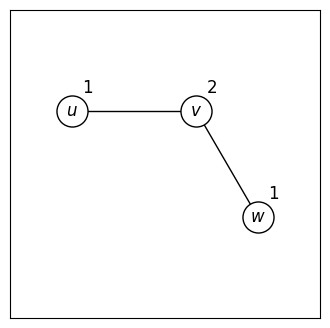
\includegraphics[width=\textwidth]{figures/lwl vs wl-ed/G1.png}
            \caption{$G_1$}
        \end{subfigure}
        \hfill
        \begin{subfigure}[b]{0.3\textwidth}
            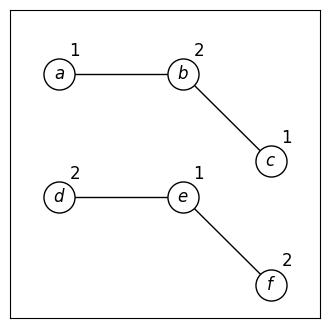
\includegraphics[width=\textwidth]{figures/lwl vs wl-ed/G2.png}
            \caption{$G_2$}
        \end{subfigure}
        \hfill
        \begin{subfigure}[b]{0.3\textwidth}
            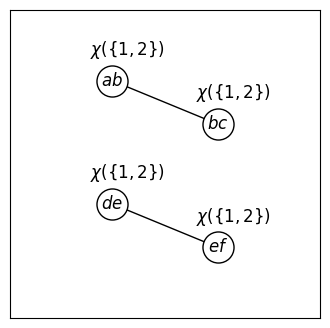
\includegraphics[width=\textwidth]{figures/lwl vs wl-ed/L(G1)-L(G2).png}
            \caption{$L(G_1)=L(G_2)$}
        \end{subfigure}
        \caption{Example of graphs $G_1$, $G_2$ that can be distinguished by $\wledge$ but not by $\lwl$.}
        \label{fig:lwl-wledge-counterexample}
    \end{figure}

    For the second part, consider the graphs $G_1$ and $G_2$ depicted in Figure \ref{fig:lwl-wledge-counterexample}.
    % TODO: draw the graphs
\end{proof}


\section{Experiments}



\section{Outlook and Conclusion}

% Extend to edge-attributed graphs
% Extend to directed graphs
% Extend to higher-order lemmas
% Extend to knowledge graphs


\bibliographystyle{unsrt}
\bibliography{refs}


\end{document}